
The aim of this proposal is to (1) identify a set of principles for
the analysis (formal, static, and dynamic) of implementations of
embedded and networked systems; (2) match these theoretical principles
with tools usable by engineers developing such systems; and (3) enable
the synergistic use of enhanced versions of these tools in real
applications through a common framework with minimal duplication of
effort and maximal extraction of information from shared annotations.
In the first case study, we will analyze networks of wireless sensor
nodes deployed in the Southwest Experimental Garden Array
(SEGA)~\cite{YamEtAl10,FliEtAl12} -- a distributed facility for
examining climatic, genetic, and environmental factors in plant
ecology -- and in the Distributed Sensing \& Computing Over Sparse
Environments (DISCOVER) Platform -- an NSF CCRI project that develops
a large-scale and diverse testbed for wireless sensor networks and
multi-robot systems.  The second case study will use the framework to
formally verify and dynamically test implementations of autonomous
control and coordination of multiple autonomous terrestrial and aerial
robots on the DISCOVER platform.

\begin{figure}[!t]
  \centering
  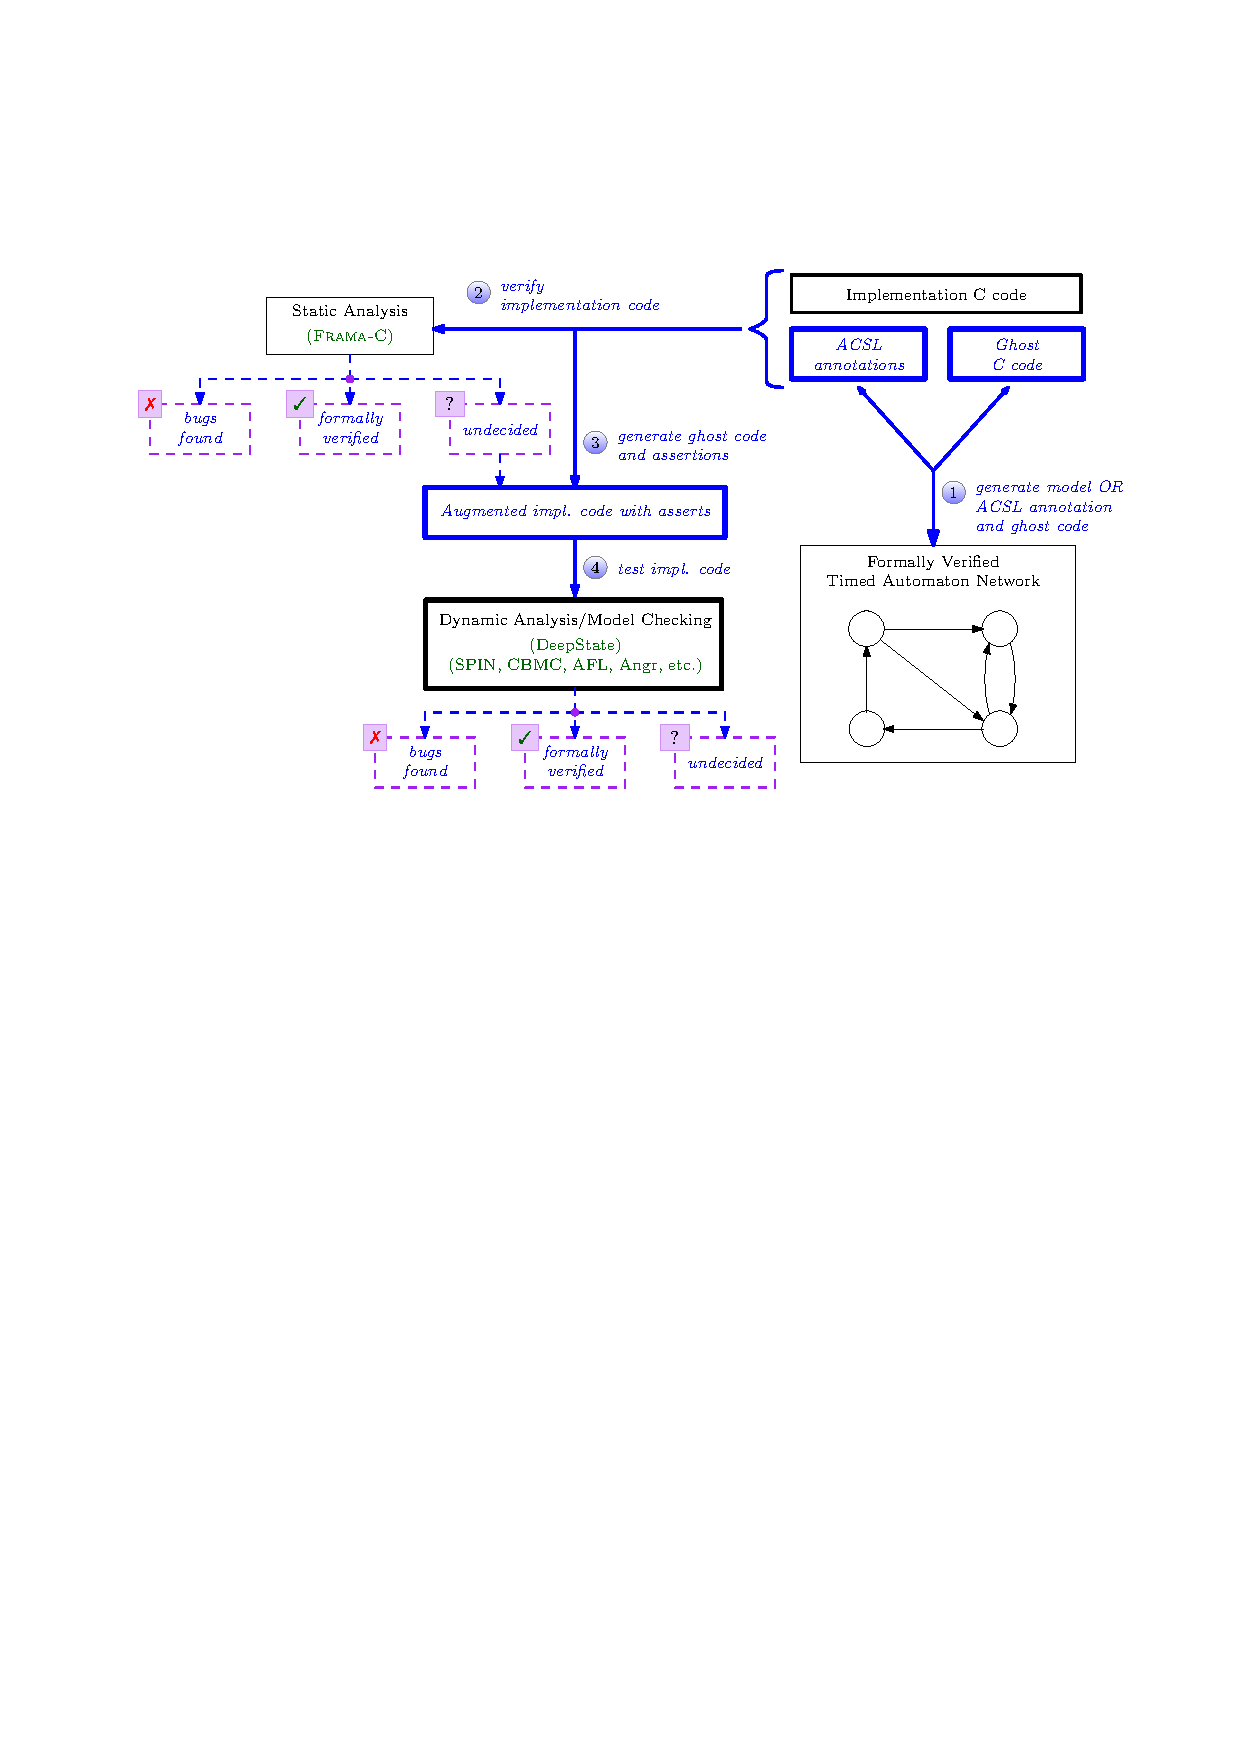
\includegraphics[width=.75\textwidth]{newoverview}
  \caption{Overview of the proposed research.\vspace{-4pt}}
  \label{fig:overview}
\end{figure}

Figure~\ref{fig:overview} shows the overall concept.  The core
open research problems addressed are represented by two sets of
arrows.  First, an engineering design, expressed as C code, is
provided, and annotated with correctness properties, information
about the expected environment (constraints on sensor values, etc.),
and hints to guide heuristic application of tools ranging from fuzzers
to symbolic execution engines to model checkers.
While they are not the focus of this project, code to apply advanced static analysis or timed
automata (TA) model skeletons can also be automatically generated:
\begin{enumerate}[labelsep=3pt,leftmargin=12pt]
\item A (generated) TA model can be used to check high-level properties
  of the design, ignoring many low-level implementation details. However, this step
  is often skipped in practice.
\item The implementation code with the \acsl annotations and ghost code
  can be checked by a static analysis tool, such as \framac.  In some
  cases this will verify the code, and in other cases a definite bug
  will be found; but often the result will be ``undecided'' and
  further analysis required to see if a bug is spurious or real.
 Again, this step can be skipped, though it is likely low-cost and beneficial.
\item Finally, the focus of our efforts is a multi-pronged attempt to refute correctness (or increase our confidence
  in it) via dynamic analysis---automated test generation---and
  implementation-level model checking.
  Ghost code, additional assertions, and needed test-harnesses are \emph{automatically generated} from 
  annotated code.
\item The augmented implementation code is then analyzed using the
  \deepstate~\cite{DeepState} framework, which serves as a front-end
  to highly scalable fuzzers, as well as to symbolic execution tools
  and model checkers.
\end{enumerate}

Our focus is on providing a unified specification method that can be
applied to source code itself, and on enabling and enhancing the dynamic analysis and
model
checking aspects of the approach.  We believe these approaches are
currently difficult to apply, but likely to
dramatically improve the ability to detect bugs.

\paragraph{Principles:} Assuming that an algorithm for an embedded and
networked system, such as a communication protocol, can in theory be
described as (probabilistic) timed automata~\cite{AD1994:TCS}, which
satisfies temporal logic formulas~\cite{BLM2017:LNCS}, and implemented
as a set of imperative programs, we ask:
\begin{itemize}[labelsep=3pt,leftmargin=12pt]
\item Given a set of annotated programs, how can we best automatically
  find bugs in those programs (and, in some circumstances, for some
  properties, prove correctness), based on an annotated
  specification?
\item Can we generate a skeleton of a timed automata model from 
  annotated programs, in order to facilitate adoption of design-level analysis by 
  traditional embedded systems developers? 
\end{itemize}
% REMOVED MENTIONS OF THE TOY LANGUAGE
%For the first problem, we will consider a toy imperative language with the
%usual control structures, unbounded integers, addresses, and
%non-recursive procedures.

Note that these problems differ considerably from the more studied,
but more limited, synthesis problem.  We are not assuming that
system development will involve first producing a formal model, then
using that model to automatically generate an implementation; rather,
we consider the typical real-world scenario, where modeling is a
separate activity, either undertaken after implementation due to
concerns about reliability, or an activity during design that only
indirectly informs the implementation.  That is, the more studied
problem is producing a runtime semantics for a model; we address the
problem of reconciling a runtime semantics with a model semantics,
without unrealistic burden on engineers.   Any
effort to increase the
adoption of formal methods and automated test generation
approaches is likely to be successful only to the extent that it enters
embedded systems engineering practice via this existing pathway.  Engineers at Google have referred to this
approach as ``meeting developers where they are''~\cite{meeting}.


\paragraph{Tools:} We will focus on C code, using \deepstate~\cite{DeepState}
as a front-end for dynamic and implementation-level model checking approaches, and
\uppaal~\cite{uppaal} and
\prism~\cite{KNP2011:CAV} for the analysis of protocols; \framac will
provide a powerful static analysis framework, and we will adopt its
\acsl language developed for \framac as a basis for our specification language.  The primary open research questions here are numerous, and include:
% (1) how to handle C constructs that are not part of the toy language;
(1) how to extend existing specification languages to support timing, interrupts,
and uncertainty;
(2) how to assign the same meaning to a specification construct in
  various contexts, ranging from fuzzing to symbolic execution to
  explicit-state model checking to bounded model checking in the
  ``dynamic'' \deepstate world, and including a static context for
  \framac and a modeling context for timed automata;
(3) how to minimize annotation burden while allowing developers to
include information that can be exploited by those methods: e.g., to
make intelligent use of pre-conditions in fuzzing, to automatically
derive loop bounds in bounded model checking, and to restrict
branching factors and store state in explicit-state model checking;
(4) how to handle intra-program parallelism;
(5) how to ensure that the methods are sufficiently automatic
  and behave in ways engineers will expect.
Our focus will be on \emph{practical} solutions, guided by domain experts, rather than on purely theoretical approaches
that do not scale. Practical solutions here require
fundamental contributions to system and specification design and
dynamic analysis and model checking technologies.

\paragraph{Field applications:}
This project will contribute significantly to the field domains of embedded and networked systems, especially in safety-critical applications where correctness and reliability are vital.
The methods and tools developed by our team will enable domain experts without formal training in formal methods and software testing, to test and verify their code to not only reduce bugs but also gain confidence in their systems.


%%% Local Variables:
%%% mode: latex
%%% TeX-master: "main"
%%% End:
